%% ----------------------------------------------------------------
%% Thesis.tex -- MAIN FILE (the one that you compile with LaTeX)
%% ---------------------------------------------------------------- 

% Set up the document
\documentclass[a4paper, 11pt, oneside]{Thesis}  % Use the "Thesis" style, based on the ECS Thesis style by Steve Gunn
\graphicspath{Figures/}  % Location of the graphics files (set up for graphics to be in PDF format)

% Include any extra LaTeX packages required
\usepackage[square, numbers, comma, sort&compress]{natbib}  % Use the "Natbib" style for the references in the Bibliography
\usepackage{verbatim}  % Needed for the "comment" environment to make LaTeX comments
\usepackage{vector}  % Allows "\bvec{}" and "\buvec{}" for "blackboard" style bold vectors in maths
\hypersetup{urlcolor=blue, colorlinks=true}  % Colours hyperlinks in blue, but this can be distracting if there are many links.

%% ----------------------------------------------------------------
\begin{document}
\frontmatter      % Begin Roman style (i, ii, iii, iv...) page numbering

% Set up the Title Page
\title  {External Kink Modes in Shaped Tokamak Plasmas}
\authors  {\texorpdfstring
            {\href{your web site or email address}{Patrick James Byrne}}
            {Patrick James Byrne}
            }
\addresses  {\groupname\\\deptname\\\univname}  % Do not change this here, instead these must be set in the "Thesis.cls" file, please look through it instead
\date       {\today}
\subject    {}
\keywords   {}

\maketitle
%% ----------------------------------------------------------------

\setstretch{1.3}  % It is better to have smaller font and larger line spacing than the other way round

% Define the page headers using the FancyHdr package and set up for one-sided printing
\fancyhead{}  % Clears all page headers and footers
\rhead{\thepage}  % Sets the right side header to show the page number
\lhead{}  % Clears the left side page header

\pagestyle{fancy}  % Finally, use the "fancy" page style to implement the FancyHdr headers

%% ----------------------------------------------------------------
% Declaration Page required for the Thesis, your institution may give you a different text to place here
\Declaration{

\addtocontents{toc}{\vspace{1em}}  % Add a gap in the Contents, for aesthetics

I, AUTHOR NAME, declare that this thesis titled, `THESIS TITLE' and the work presented in it are my own. I confirm that:

\begin{itemize} 
\item[\tiny{$\blacksquare$}] This work was done wholly or mainly while in candidature for a research degree at this University.
 
\item[\tiny{$\blacksquare$}] Where any part of this thesis has previously been submitted for a degree or any other qualification at this University or any other institution, this has been clearly stated.
 
\item[\tiny{$\blacksquare$}] Where I have consulted the published work of others, this is always clearly attributed.
 
\item[\tiny{$\blacksquare$}] Where I have quoted from the work of others, the source is always given. With the exception of such quotations, this thesis is entirely my own work.
 
\item[\tiny{$\blacksquare$}] I have acknowledged all main sources of help.
 
\item[\tiny{$\blacksquare$}] Where the thesis is based on work done by myself jointly with others, I have made clear exactly what was done by others and what I have contributed myself.
\\
\end{itemize}
 
 
Signed:\\
\rule[1em]{25em}{0.5pt}  % This prints a line for the signature
 
Date:\\
\rule[1em]{25em}{0.5pt}  % This prints a line to write the date
}
\clearpage  % Declaration ended, now start a new page

%% ----------------------------------------------------------------
% The "Funny Quote Page"
\pagestyle{empty}  % No headers or footers for the following pages

\null\vfill
% Now comes the "Funny Quote", written in italics
\textit{``Write a funny quote here.''}

\begin{flushright}
If the quote is taken from someone, their name goes here
\end{flushright}

\vfill\vfill\vfill\vfill\vfill\vfill\null
\clearpage  % Funny Quote page ended, start a new page
%% ----------------------------------------------------------------

% The Abstract Page
\addtotoc{Abstract}  % Add the "Abstract" page entry to the Contents
\abstract{
\addtocontents{toc}{\vspace{1em}}  % Add a gap in the Contents, for aesthetics

The Thesis Abstract is written here (and usually kept to just this page). The page is kept centered vertically so can expand into the blank space above the title too\ldots

}

\clearpage  % Abstract ended, start a new page
%% ----------------------------------------------------------------

\setstretch{1.3}  % Reset the line-spacing to 1.3 for body text (if it has changed)

% The Acknowledgements page, for thanking everyone
\acknowledgements{
\addtocontents{toc}{\vspace{1em}}  % Add a gap in the Contents, for aesthetics

The acknowledgements and the people to thank go here, don't forget to include your project advisor\ldots

}
\clearpage  % End of the Acknowledgements
%% ----------------------------------------------------------------

\pagestyle{fancy}  %The page style headers have been "empty" all this time, now use the "fancy" headers as defined before to bring them back


%% ----------------------------------------------------------------
\lhead{\emph{Contents}}  % Set the left side page header to "Contents"
\tableofcontents  % Write out the Table of Contents

%% ----------------------------------------------------------------
\lhead{\emph{List of Figures}}  % Set the left side page header to "List if Figures"
\listoffigures  % Write out the List of Figures

%% ----------------------------------------------------------------
\lhead{\emph{List of Tables}}  % Set the left side page header to "List of Tables"
\listoftables  % Write out the List of Tables

%% ----------------------------------------------------------------
\setstretch{1.5}  % Set the line spacing to 1.5, this makes the following tables easier to read
\clearpage  % Start a new page
\lhead{\emph{Abbreviations}}  % Set the left side page header to "Abbreviations"
\listofsymbols{ll}  % Include a list of Abbreviations (a table of two columns)
{
% \textbf{Acronym} & \textbf{W}hat (it) \textbf{S}tands \textbf{F}or \\
\textbf{LAH} & \textbf{L}ist \textbf{A}bbreviations \textbf{H}ere \\

}

%% ----------------------------------------------------------------
\clearpage  % Start a new page
\lhead{\emph{Physical Constants}}  % Set the left side page header to "Physical Constants"
\listofconstants{lrcl}  % Include a list of Physical Constants (a four column table)
{
% Constant Name & Symbol & = & Constant Value (with units) \\
Speed of Light & $c$ & $=$ & $2.997\ 924\ 58\times10^{8}\ \mbox{ms}^{-\mbox{s}}$ (exact)\\

}

%% ----------------------------------------------------------------
\clearpage  %Start a new page
\lhead{\emph{Symbols}}  % Set the left side page header to "Symbols"
\listofnomenclature{lll}  % Include a list of Symbols (a three column table)
{
% symbol & name & unit \\
$a$ & distance & m \\
$P$ & power & W (Js$^{-1}$) \\
& & \\ % Gap to separate the Roman symbols from the Greek
$\omega$ & angular frequency & rads$^{-1}$ \\
}
%% ----------------------------------------------------------------
% End of the pre-able, contents and lists of things
% Begin the Dedication page

\setstretch{1.3}  % Return the line spacing back to 1.3

\pagestyle{empty}  % Page style needs to be empty for this page
\dedicatory{For/Dedicated to/To my\ldots}

\addtocontents{toc}{\vspace{2em}}  % Add a gap in the Contents, for aesthetics


%% ----------------------------------------------------------------
\mainmatter	  % Begin normal, numeric (1,2,3...) page numbering
\pagestyle{fancy}  % Return the page headers back to the "fancy" style

% Include the chapters of the thesis, as separate files
% Just uncomment the lines as you write the chapters

\chapter{Introduction}
\indent The world faces a series of stark choices in the coming years.  The warming of the earth continues to rise, and the rise to accelerate.  As of this writing it is 68$^{\circ}$F and it is also mid-December.  Though there are a series of entrenched interests that resist acknowledging the facts as such, the use of fossil fuels forcing the change is settled science.  However, human development is inextricably linked to the exploitation of energy.  The environmental disruption caused by China's rapid development in the last quarter century is merely an amplified echo of that experienced by the western world during the industrial revolution.  There remain billions of people on earth living in places that have yet to develop, and though raising them to the standard of life enjoyed by the first world would multiply the current consumption of fossil fuels by several times we have no moral right to deny them the lifestyle we enjoy.\par
Given that the use of fossil fuel is already exponentially increasing, and that they are created at a rate many orders of magnitude slower than we are exploiting them, one way or another, at some point in the future, it is guaranteed that humanity will no longer be using fossil fuels to power itself, though that replacement may be wood, peat, or dung, if a more suitable replacement is not found.\par
Carbon-Neutral power generation is thus a must if we are to progress as a species.  The localised, seasonalised and intermittent generation from most renewables disqualifies them until and unless power storage and public grids can catch up.  Hydroelectric is environmentally damaging, and as demonstrated by California's recent drought, subject to the extreme weather caused by global warming.  Nuclear accidents have cost far less in terms of human morbidity than the chronic effects due to burning coal, but the poor public understanding of the physics and technology involved, and the spectacularity with which the failures occur, has made it extremely controversial.\par
Fusion energy is the path out of the bind we find ourselves in with a better future at the end.  The fusion products do not contribute to the greenhouse effect.  The generation is not dependent on seasons or weather.  There is no possibility for a runaway meltdown reaction, and as a new technology with a high degree of enthusiasm among the public, it has none of the perception issues attached to fission nuclear.  One component of the fuel, the hydrogen isotope deuterium, is abundant, with reserves to last several thousands of years.  It is widely distributed, reducing the pressures that lead to conflict over resources.    Though the containment vessel will become activated and radioactive, much like current fission reactors, the reaction products will not be nuclear waster.  Further, there exist more advanced fuel mixes that are completely aneutronic, removing even that slight drawback.  Harnessing fusion is not just a scientific and technical challenge, it is a moral imperative.

\section{The D-T Fusion Reaction}
Fusion occurs if two ions collide with enough energy to overcome the coulomb repulsion of their nuclei until they can come close enough for the strong force interaction to take over, merging the two nuclei.  Different reactions between different reactants and occur at different temperatures, and have larger or smaller cross sections.  The larger the cross section, the smaller the confinement time, or the lower the density required for a certain number of reactions to occur.  Given that the ions in a plasma have a distriubtion of temperatures, the figure of merit for energy generation in a fusion plasma is the value of the so called 'triple product':\begin{equation}
nT\tau_E \geq 5*10^{21} \frac{keV\cdot s}{m^3}
\end{equation} with n being the particle density of the plasma, $\tau_E$ being the energy confinement time, and T being the plasma temperature.  The minimum value in the inequality is for the reaction between deuterium and tritium, which, as the least technically demanding fusion reaction, is the main focus of fusion research.  The values of relevance to tokamak fusion are $T \simeq 10keV$, $n \simeq 10^{20}m^{-3}$, $\tau_E \simeq  5s$ This reaction creates a neutron and a helium-4, or alpha, ion:\begin{equation}
D+T \rightarrow \alpha(3.5MeV) + n(14.3 MeV)
\end{equation}

The magnetically confined helium 'ash' heats the plasma as it thermalizes, and the unconfined neutron carries its heat out of the plasma.  The neutrons are captured in a 'blanket' that absorbs the heat and transfers it to a coolant to generate power.  The blanket can also be given a lithium coating, which on absorption of a neutron generates tritium, helium, and additional energy.\par
\section{Plasma Confinement}
The temperatures required for fusion are above $10^6 K$.  This is far higher than the melting temperature of any available material.  There is therefore a need for a strong temperature gradient between the fusion plasma and any chamber that will contain it.  Diffusion of the plasma, and thus heat transport can be slowed significantly by imposition of a magnetic field in the plasma.  This field will exert a Lorentz force 
\begin{equation}
\vec{F} = q(\vec{E} + \vec{v} \times \vec{B}) 
\end{equation}
on particles moving perpendicular to the direction of the magnetic field.  Viewed along a magnetic field line, charged particles will trace circles of smaller and smaller radii as the field strength is increased.  This radius, known as the Larmor radius, is defined as:\begin{equation}
r_L = \frac{mv_\perp}{qB}
\end{equation}
with m the particle's mass, $v_\perp$ the component of the velocity perpendicular to the magnetic field, q the particle's charge, and B the magnetic field strength.
There is, however, no force felt by a particle traveling along a field line, and so confinement of a plasma in three dimensions is not achievable with straight, uniform magnetic fields.  In tokamaks, an electromagnet generates circular magnetic fields, which is referred to as the toroidal magnetic field.  Plasma is thus free to travel in a periodic fashion along the circular field lines, with diffusion of plasma in a radial direction strongly suppressed.  Plasma diffusion in a vertical direction is also suppressed, but there will be a drift of bulk plasma upwards.  This is due to a net drift of the plasma either up or downwards, caused by the radial gradient in the toroidal field strength.  To counteract this drift, it is necessary to impose a second magnetic field on the plasma.\par 
In tokamaks, this is primarily achieved by passing a large current through the plasma.  This current will add a magnetic field, referred to as the poloidal field, that encircles the plasma.  The resultant field traces a helix through space, and as a plasma element follows this field line the drift will be canceled on average.\par
\subsection{Efficiency and $\beta$}
Generating the toroidal and poloidal fields requires an input of energy, which in a fuison power plant would be deducted against the energy generated.  Given that the rate of energy generation is related to density and pressure, as in Eq \eqref{1}, a useful figure of merit for the efficiency of a fusion power plant is $\beta$, or the ratio of confined plasma pressure to the pressure of the confining magnetic field.  $\beta$ can be expressed with respect to either the toroidal or poloidal magnetic field:
\begin{eqnarray}	
\beta_t = \frac{\langle p \rangle}{\langle B_t \rangle^2/2\mu_0}\\
\beta_p = \frac{\langle p \rangle}{\overline{B}_p^2/2\mu_0}
\end{eqnarray}
Where quantities in brackets $\langle x \rangle$ are the volume averaged, p is the plasma pressure, $B_t$ is the toroidal magnetic field, $\overline{B}_p$ defined as $\frac{\mu_0 I_P}{2 \pi a \kappa}$. The elongation $\kappa$ defined as $\frac{A}{\pi a^2}$ with A the cross-sectional area of the plasma. Further, $\beta_t$ can be normalized against the plasma current, $I_p$, the minor radius $a$, \begin{equation}
\beta_N = \frac{\beta_t a B_t}{I_p}
\end{equation} % Introduction

%\chapter{HBT-EP Capabilities}
\paragraph{} The world faces a series of stark choices in the coming years.  The warming of the earth continues to rise, and the rise to accelerate.  As of this writing it is 68$^{\circ}$F and it is also mid-December.  Though there are a series of entrenched interests that resist acknowledging the facts as such, the use of fossil fuels forcing the change is settled science.  However, human development is inextricably linked to the exploitation of energy.  The environmental disruption caused by China's rapid development in the last quarter century is merely an amplified echo of that experienced by the western world during the industrial revolution.  There remain billions of people on earth living in places that have yet to develop, and though raising them to the standard of life enjoyed by the first world would multiply the current consumption of fossil fuels by several times we have no moral right to deny them the lifestyle we enjoy.  
\paragraph{}
Given that the use of fossil fuel is already exponentially increasing, and that they are created at a rate many orders of magnitude slower than we are exploiting them, one way or another, at some point in the future, it is guaranteed that humanity will no longer be using fossil fuels to power itself, though that replacement may be wood, peat, or dung, if a more suitable replacement is not found.
\paragraph{}
Carbon-Neutral power generation is thus a must if we are to progress as a species.  The localised, seasonalised and intermittent generation from most renewables disqualifies them until and unless power storage and public grids can catch up.  Hydroelectric is environmentally damaging, and as demonstrated by California's recent drought, subject to the extreme weather caused by global warming.  Nuclear accidents have cost far less in terms of human morbidity than the chronic effects due to burning coal, but the poor public understanding of the physics and technology involved, and the spectacularity with which the failures occur, has made it extremely controversial.
\paragraph{}
Fusion energy is the path out of the bind we find ourselves in with a better future at the end.  The fusion products do not contribute to the greenhouse effect.  The generation is not dependent on seasons or weather.  There is no possibility for a runaway meltdown reaction, and as a new technology with a high degree of enthusiasm among the public, it has none of the perception issues attached to fission nuclear.  One component of the fuel, the hydrogen isotope deuterium, is abundant, with reserves to last several thousands of years.  It is widely distributed, reducing the pressures that lead to conflict over resources.    Though the containment vessel will become activated and radioactive, much like current fission reactors, the reaction products will not be nuclear waster.  Further, there exist more advanced fuel mixes that are completely aneutronic, removing even that slight drawback.  Harnessing fusion is not just a scientific and technical challenge, it is a moral imperative.

\section{The D-T Fusion Reaction}
\paragraph{}
Fusion occurs if two ions collide with enough energy to overcome the coulomb repulsion of their nuclei until they can come close enough for the strong force interaction to take over, merging the two nuclei.  Different reactions between different reactants and occur at different temperatures, and have larger or smaller cross sections.  The larger the cross section, the smaller the confinement time, or the lower the density required for a certain number of reactions to occur.  Given that the ions in a plasma have a distriubtion of temperatures, the figure of merit for energy generation in a fusion plasma is the value of the so called 'triple product':\begin{equation}
nT\tau_E \geq 5*10^{21} \frac{keV\cdot s}{m^3}
\end{equation} with n being the particle density of the plasma, $\tau_E$ being the energy confinement time, and T being the plasma temperature.  The minimum value in the inequality is for the reaction between deuterium and tritium, which, as the least technically demanding fusion reaction, is the main focus of fusion research.  The values of relevance to tokamak fusion are $T \simeq 10keV$, $n \simeq 10^{20}m^{-3}$, $\tau_E \simeq  5s$ This reaction creates a neutron and a helium-4, or alpha, ion:\begin{equation}
D+T \rightarrow \alpha(3.5MeV) + n(14.3 MeV)
\end{equation}

The magnetically confined a helium 'ash' heats the plasma as it thermalizes, and the unconfined neutron carries its heat out of the plasma.  The neutrons are captured in a 'blanket' that absorbs the heat and transfers it to a coolant to generate power or can be captured by a lithium coating, generating tritium, helium, and additional energy.
\paragraph{}
It is not enough, however to merely generate energy.  More energy must be generated than was used to heat and confine the plasma, and the imbalance must be large enough that the excess can be sold at a low enough cost to be competitive, and at high enough volume to underwrite the operation of the plant and provide a profit for the operators.  The most common measurement of tokamak efficiency is $\beta$, which is the ratio of the plasma pressure to magnetic pressure.  $\beta$ can be expressed with respect to either the toroidal or poloidal magnetic field, or the combination:
\begin{eqnarray}	
\beta_t = \frac{\langle p \rangle}{\langle B_t \rangle^2/2\mu_0}\\
\beta_p = \frac{\langle p \rangle}{\overline{B}_p^2/2\mu_0}
\end{eqnarray}
Where $\langle p \rangle$ is the volume averaged plasma pressure, $B_t$ is the toroidal magnetic field, $B_p$ is the poloidal magnetic field,Further, $\beta_t$ can be normalized against the plasma current, $I_p$, the minor radius $a$, \begin{equation}
\beta_N = \frac{\beta_T a B_t}{I_p}
\end{equation}
\section{plasma confinement}

\subsection{A Subsection}

Donec urna leo, vulputate vitae porta eu, vehicula blandit libero. Phasellus eget massa et leo condimentum mollis. Nullam molestie, justo at pellentesque vulputate, sapien velit ornare diam, nec gravida lacus augue non diam. Integer mattis lacus id libero ultrices sit amet mollis neque molestie. Integer ut leo eget mi volutpat congue. Vivamus sodales, turpis id venenatis placerat, tellus purus adipiscing magna, eu aliquam nibh dolor id nibh. Pellentesque habitant morbi tristique senectus et netus et malesuada fames ac turpis egestas. Sed cursus convallis quam nec vehicula. Sed vulputate neque eget odio fringilla ac sodales urna feugiat.

\section{Another Section}

Phasellus nisi quam, volutpat non ullamcorper eget, congue fringilla leo. Cras et erat et nibh placerat commodo id ornare est. Nulla facilisi. Aenean pulvinar scelerisque eros eget interdum. Nunc pulvinar magna ut felis varius in hendrerit dolor accumsan. Nunc pellentesque magna quis magna bibendum non laoreet erat tincidunt. Nulla facilisi.

Duis eget massa sem, gravida interdum ipsum. Nulla nunc nisl, hendrerit sit amet commodo vel, varius id tellus. Lorem ipsum dolor sit amet, consectetur adipiscing elit. Nunc ac dolor est. Suspendisse ultrices tincidunt metus eget accumsan. Nullam facilisis, justo vitae convallis sollicitudin, eros augue malesuada metus, nec sagittis diam nibh ut sapien. Duis blandit lectus vitae lorem aliquam nec euismod nisi volutpat. Vestibulum ornare dictum tortor, at faucibus justo tempor non. Nulla facilisi. Cras non massa nunc, eget euismod purus. Nunc metus ipsum, euismod a consectetur vel, hendrerit nec nunc. % Background Theory 

%\chapter{Shaping on HBT-EP}
\section{Hardware}
\subsection{The Coil}
\paragraph{} The shaping coil is a single continuous piece of 1/0 welding cable, run eight times toroidally between the inner ring of the toroidal field magnet cases and the vacuum vessel.  This ex-vessel coil is located slightly above the midplane, mainly due to space limitations.  Were there complete freedom of placement, the coil would likely be placed nearer the midplane, as we have active (pre-programmed) control of the plasma's radial location, but vertical location control is only passively provided by eddies in the conducting vessel walls and shells.  Further, placing the coil at the midplane would locate it closer the the plasma, increasing coupling and reducing the current requirements for any given shape
\subsubsection{Leads \& Bundle Connections} 
The construction of the coil out of a single conductor was accomplished through directing the conductor from one bundle to another once the number of required turns had been wound.  This necessitated a poloidal run of wire to connect the two.  At the end of the final bundle, the out-lead cable had to travel poloidally once again to meet the in-lead before becoming a twisted pair.  These non-toroidal runs of current were canceled to the best of our ability by running the return lead back at the same location as the poloidal leads connecting each bundle.  Though the thickness of the cable and the tight spaces involved precluded winding these contrary wires, they were connected with zip ties to ensure as good a canceling as possible.  See Figure 1 for a schematic of the windings and location of the leads.\\
\begin{figure}
\includegraphics[width = \textwidth]{./figures/Coil_winding_schematic.png}\begin{flushleft}
\caption{Schematic of the current direction, inter-bundle connections and coil leads, as seen by an observer between the vacuum vessel's inboard side and the coil.  The toroidal direction is left/right, poloidal is up/down.}
\end{flushleft}
\label{coil_winding}
\end{figure}
The twisted pair from the power supply rises from the laboratory basement, splits with one lead breaking into the lowest turn, and the other breaking out of the highest turn.  The top lead is therefore unshielded for roughly 8 inches.  There are two points at which the cable is bent back upon itself to begin a new bundle and reverse the direction of the current.  This occurs at the same toroidal location, which is itself the same location as the leads.  The current in the leads travels in the opposite direction from the current in the jumps between bundles.  The lead is thus lashed to the the interbundle connections to both reduce the error fields, and prevent the $\vec{j} X \vec{B}$ forces on the cables from causing damage to the coil insulation.
\subsubsection{The Power Supply}
\paragraph{}The shaping coil is energized by a pre-programmed two-stage passive capacitive supply.  A 7.5mF, 900V (max) bank provides the startup current, with a time to peak current of $800\mu s$.  As this bank discharges, a high current diode passively switches a second 'crowbar' bank into the circuit.  This bank has a capacitance of 0.6F, and a maximum voltage of 250V.  This much larger bank is capable of providing current enough to sustain a 'flat top' current pulse of $\sim$8kA for $\sim$5ms.  By selecting different voltages on each bank pre-discharge, a variety of different current profiles can be developed.  The 'soft start' of the crowbar bank due to the used of a diode allows for a very smooth transition between the two power banks.  This is compared to the current trace of the vertical field coil in Figure .  The power supplies for all other equilibrium field coils are capacitive in nature, but are switched in by ignitrons, which require a voltage drop between the bank and the line into which they switch the bank.  The rapid inrush current as a capacitor is switched into a line of a different voltage leads to a sharp change in the current, leading to strong eddies induced in the surrounding conducting structures.  The banks are easily charged to their full voltage in less than one minute, much less time than the other equilibirum field coil banks.  There are a variety of safety measures used in the bank's construction.  A discussion, full partslist and circuit schematic can be found in Appendix BLANK
\subsubsection{The Coil Holders}
The coil is supported against gravity and Lorentz forces by a set of ten  G-10 fiberglass/epoxy composite supports, which are themselves bolted to the TF cases.  The bolts are structural bolts, that had been used to clamp the TF cases shut.  Nuts located at the point of attachment have been removed, and the bolts instead thread into tapped holes in the supports.  The previous torque of 40 ft-lbs is applied, with no ill effects on the G-10 holder mounts, thus providing the same clamping force and avoiding any leaks of insulating oil.
These holders consist of two parts epoxied together, and thus do not disassemble.  The holders were attached to the Tokamak, and the coil was threaded sequentially through each hole in each conductor.  As such, any modifications or repairs to the coil or any locations on the tokamak obstructed by the coil will require the coil to be cut, or completely unwound.  Unwinding represents 2-3 business days of work, but cutting may make it difficult to splice and insulate the coil given the tight confines of its run.
The coil holders are further supplemented by a set of ten clamps, which hang from the coil itself.  Though they provide no resistance to gravity or external magnetic forces, they do prevent the coil's bundles from jumping apart due to the magnetic repulsion between the oppositely-directed bundles.
\subsubsection{Rip-testing of Coil Jump-out}
 
\subsubsection{The Material Limiter}
\paragraph{}The poloidal array sensors are protected by $\frac{1}{16}$'' stainless steel shimstock to protect against damage to the wires or ablation of the plastic forms by plasma impinging.  Under normal operating conditions the last closed flux surface of the plasma is 5mm radially inward from the surface of the sensors' shielding.  The plasma is in general vertically centered on the midplane, moves mostly radially, and disrupts inward, so sensors at the midplane are further protected by the inboard limiter, which establish a 5mm separation between plasma and sensors, and have much larger thermal mass than the shims that cover the sensors.
\paragraph{}However, this is not the case for sensors higher up that are near the location of the X-point.  These sensors which lack the extra protection of a limiter will see the steady state power flux increase as plasma will be preferentially exhausted along a cone expanding radially outward from the X-point.  Additionally, during disruptions, there will be an upward component to the forces on the plasma.  To ensure that this additional heat load does not cause harm to the sensors, a new set of 1/4" 316 stainless steel limiters was machined and installed.  These 'blade' limiters are attached by hex nuts to threaded rods spot welded to the flanges of the chamber pieces.  These limiters trace an arc concentric with the poloidal array sensors, and extend radially inward 5mm from the inner edge of the sensors.  Protection from plasma impingement is provided from $180^{\circ} \leq \Theta \geq 120^{\circ}$.

\begin{figure}
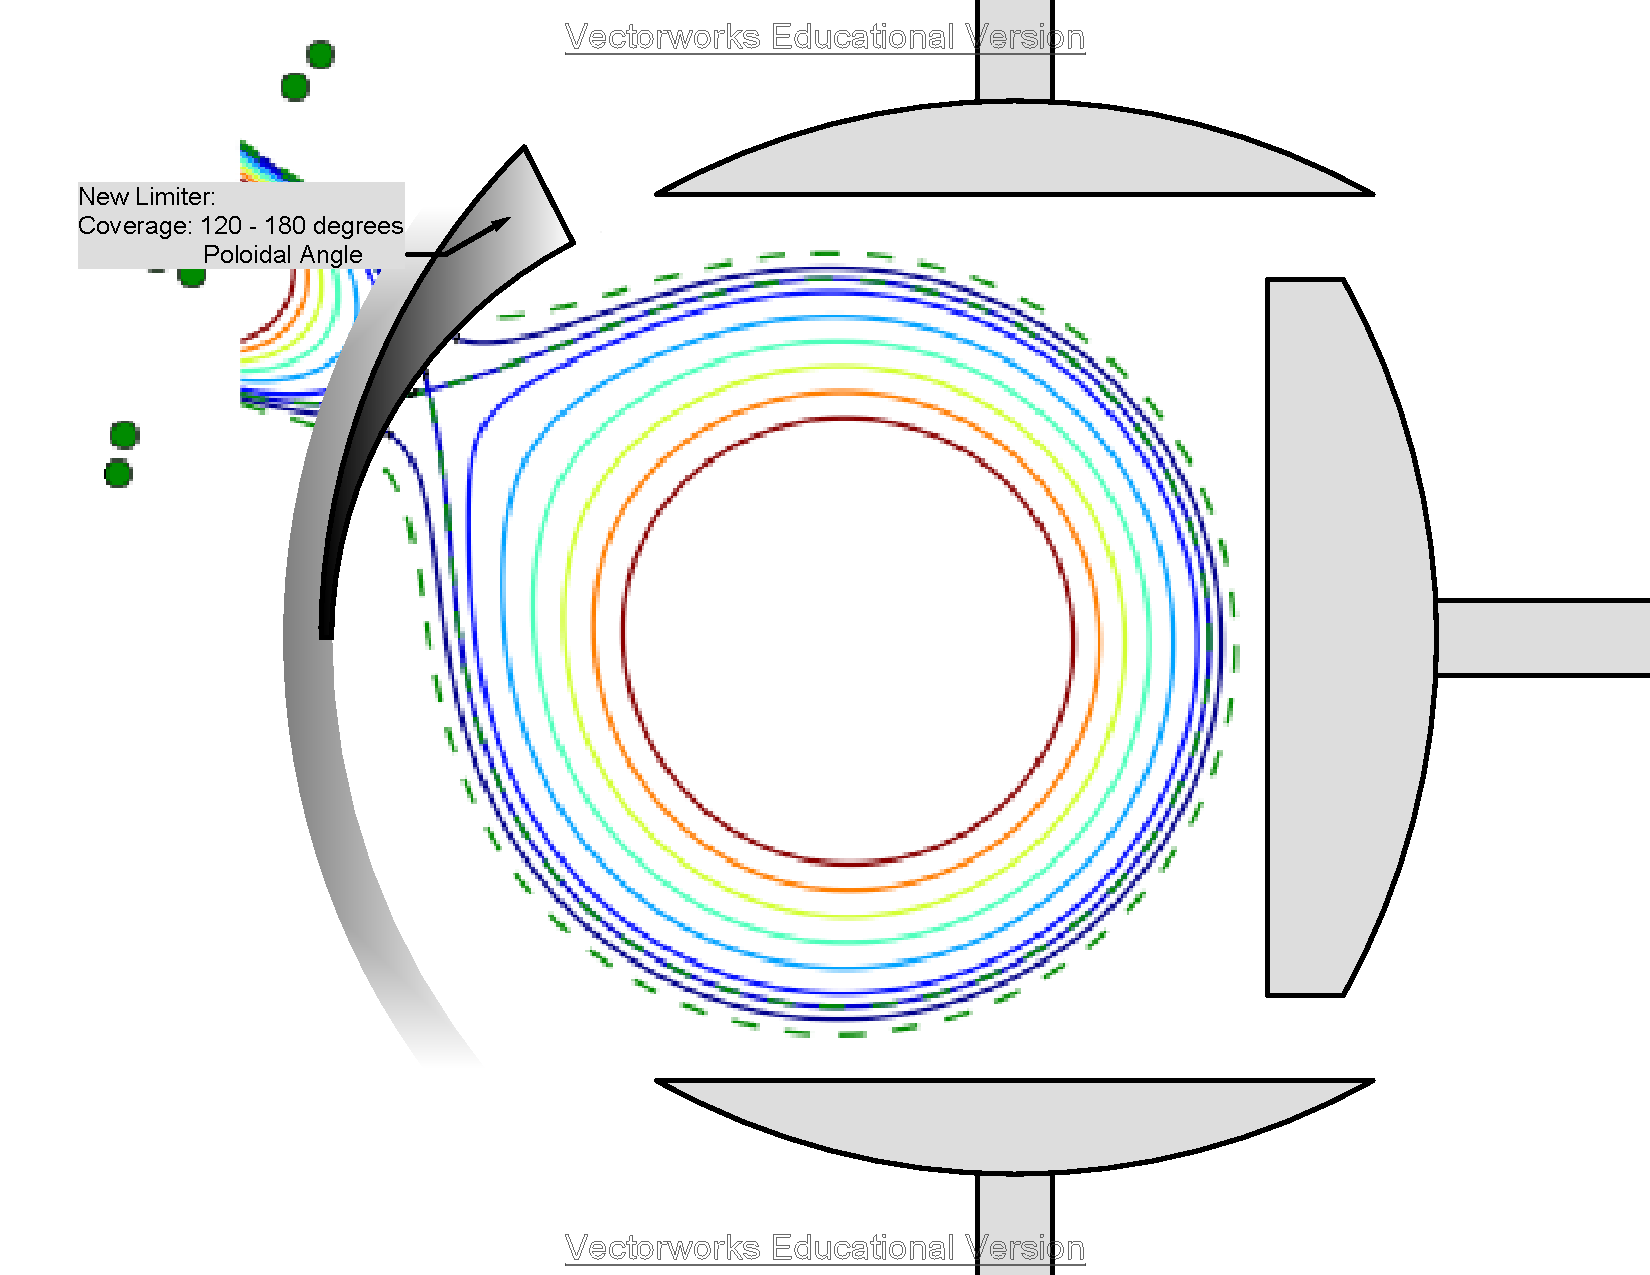
\includegraphics[width = \textwidth]{./figures/Poloidal_Cross_Section_shaping_plus_new_limter_v2013.pdf}\begin{flushleft}
\caption{Poloidal cross section of shaped plasma in chamber and limiting surfaces, with new limiter included.  Limiter is designed to to be conformal to a 15cm minor radius, inboard limited plasma.}
\end{flushleft}
\label{new_limiters}
\end{figure}

\subsection{Defining the Plasma Shape}
The definitions set out in \cite{Luce} will be used for discussion of the plasma shape in this research.  These definitions are more suited to the HBT-EP plasma, since the shaped equilibrium has no symmetry in the R-Z plane.  Common figures of merit, such as elongation and triangularity, can be defined for arbitrary geometries, and an analytic form for the LCFS can be derived.

The plot below shows a circular HBT-EP plasma, and a diverted plasma, with other equilibrium parameters (MR, I$_p$ being held constant)  % Experimental Setup

%\chapter{Signal Analysis}
\paragraph{}  The large number of sensors and the rapid sampling of each sensor provides an enormous number of individual measurements of magnetic fields during the plasma's lifetime. The method of Biorthogonal Decomposition is used to isolate coherent fluctuations from this large dataset and provides an orthogonal basis set of modes, that are described in terms of their spatial shape and temporal evolution.  This chapter will describe the method of Biorthogonal Decomposition, how it is applied in this research, its strengths and limitations.

\section{The Biorthogonal Decomposition Algorithm}
\paragraph{}
The biorthogonal decomposition is used on non-square matrices, to produce a basis set of pseudo-eigenvalues and pseudo-eigenvectors.  A given matrix S is decomposed into 
\begin{equation}
A^{\intercal} A = U \Sigma V^{\intercal}
\end{equation}
Where the columns of U and the rows of V are orthogonal bases of the structures, however defined, that make up the rows and columns of the data. In this research, the rows are time series of individual sensor signals, with the signal across all sensors at any instant constituting the columns.  
$$
\begin{pmatrix}
\uparrow& &\uparrow\\
s_1&\cdots&s_N\\
\downarrow & &\downarrow
\end{pmatrix}
 =
\begin{pmatrix}
\uparrow& &\uparrow\\
u_1&\cdots&u_N\\
\downarrow & &\downarrow
\end{pmatrix}
\begin{pmatrix}
\sigma_1& &\\
&\ddots&\\
& &\sigma_N
\end{pmatrix}
\begin{pmatrix}
\leftarrow& v_1&\rightarrow\\
&\vdots&\\
\leftarrow& v_M &\rightarrow
\end{pmatrix}
$$



  can be derived by first multiplying the vector by its transpose.  The resulting matrix is square and is factorable into two independent sets of eigenvectors, which are related to the arrangement of column and row vectors.  
In the case of HBT-EP, the time-domain signal for each sensor is stitched together to give a matrix that has dimensions up to 216 X 5000.  There will be a set of eigenvalues equal in size to the smaller dimension.  The set of eigenvectors will be determined arbitrarily, with no a priori assumptions as to the form of the basis functions.  The only constraint is that they must all be orthogonal in both space and time.  That the poloidal modes do not form a clean Fourier basis set is therefore of no concern.  The toroidal and temporal structure, for which sinusoids are a good description, will allow for orthogonal bases which map well onto individual modes regardless of poloidal structure.  Thus modes with non-singular poloidal spectra can be adequately modeled, which would not be the case if a Fourier basis was used.
As seen in figure \ref{PA_sensors_top_3_modes} The signal of all sensors in a poloidal array is put through the BD, with the top three modes isolated.  The (exxagerated) amplitude is plotted on a poloidal cross section.  The development of each mode is clear, with some modes growing as time goes on, and others declining in amplitude.  The remaining signal shows some high wavenumber, low amplitude structure, but analysis of such low level signal can be difficult.


\begin{figure}
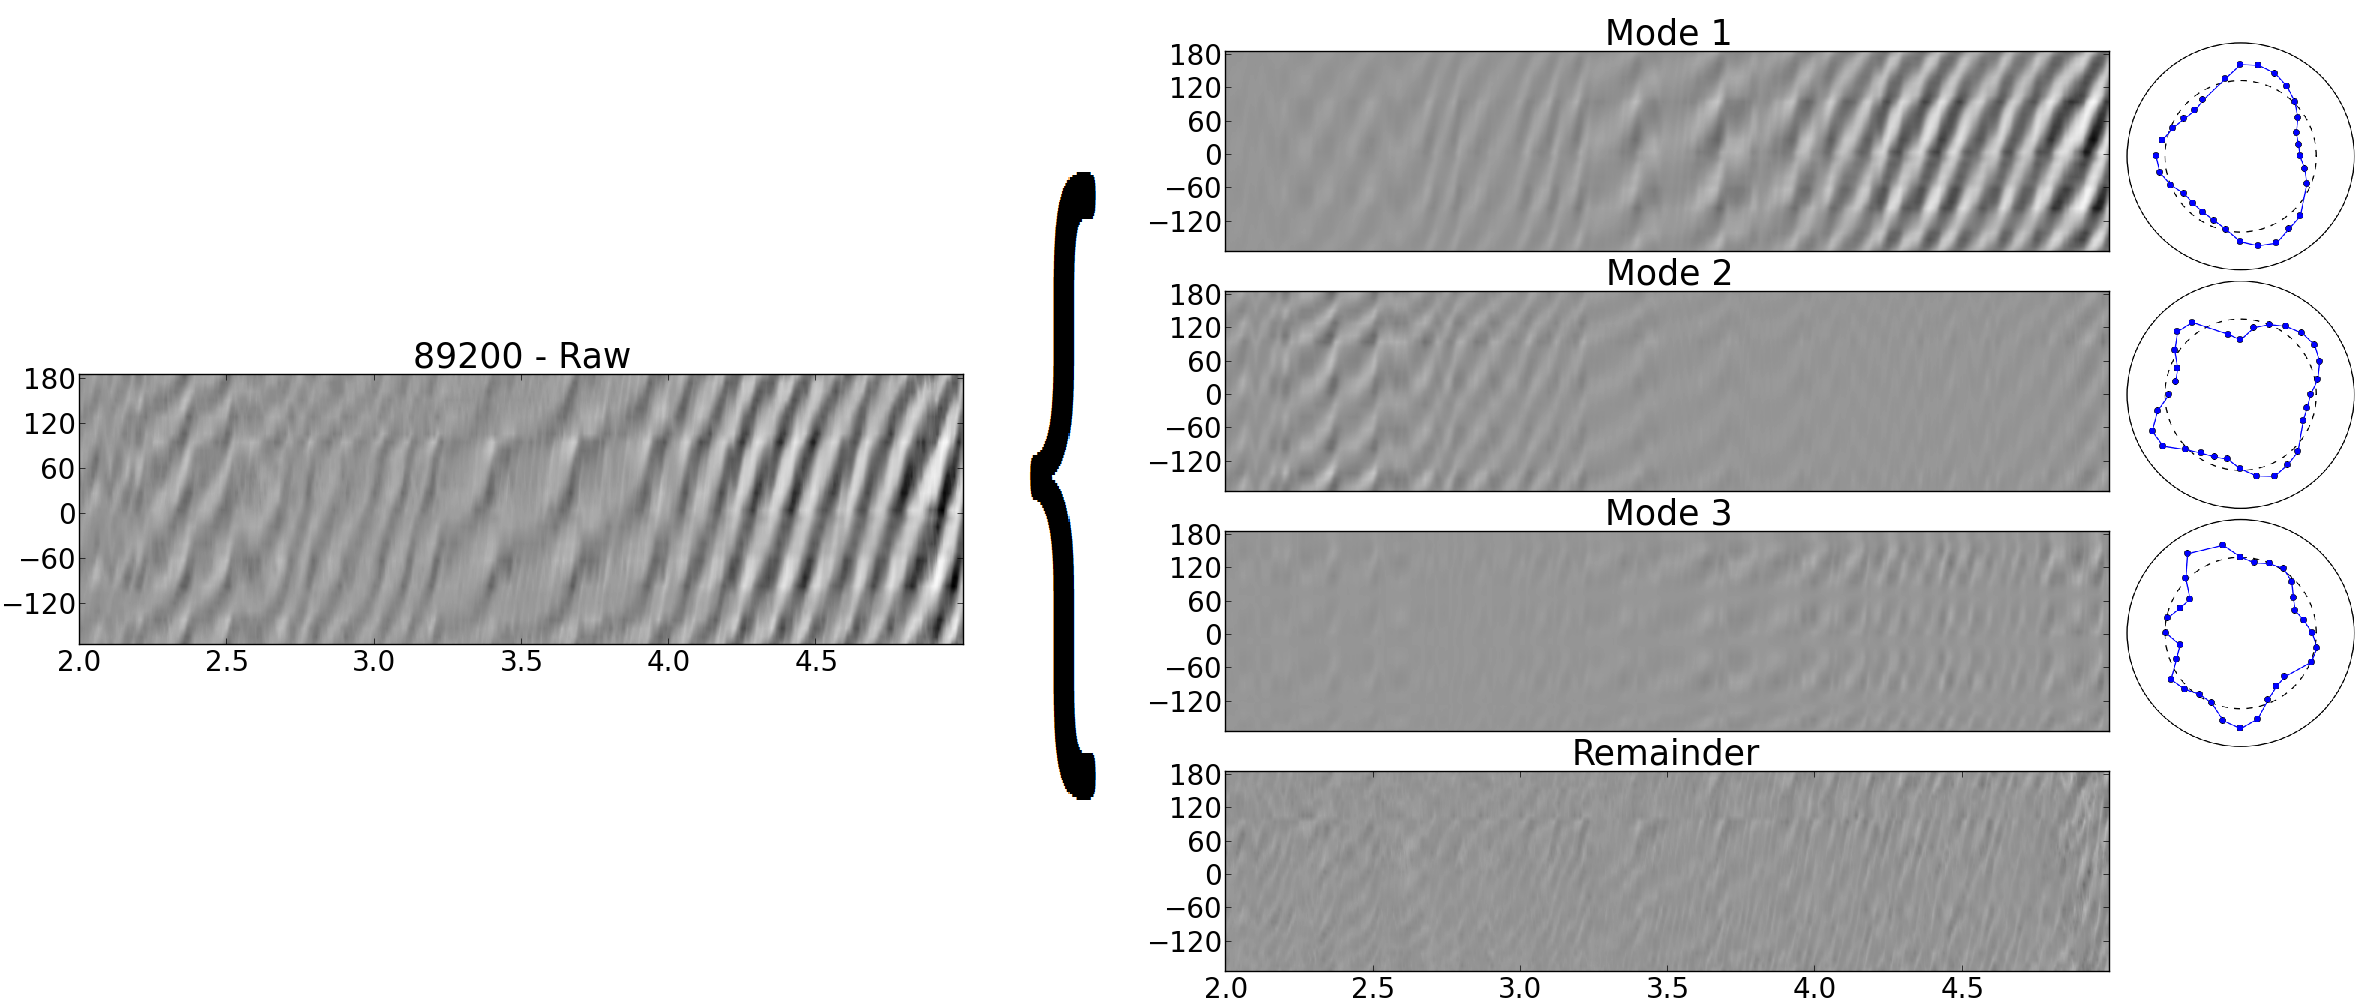
\includegraphics[width = \textwidth]{./figures/stripey_flucts_joined_grey_89200_mod.png}\begin{flushleft}
\caption{Greyscale contour plot of poloidal array raw signal, 3 dominant modes, and remainder of the full signal.  Mode structure is clearly visible, as is temporal evolution of mode amplitude.  Remainder shows structure - determining significance of low-order modes requires close analysis on a shot-by-shot basis}
\end{flushleft}
\label{PA_sensors_top_3_modes}
\end{figure}

 % Experiment 1

%\chapter{External Kink Modes in Shaped Plasmas}
\paragraph{} Shaped plasmas were developed with major radius outside 92 cm to take advantage of the modeled reduction of minor radius on the outboard side.  This allowed for a more suitable positioning of the X-point, further away from the inner walls of the chamber.
\paragraph{}
Given that the use of fossil fuel is already exponentially increasing, and that they are created at a rate many orders of magnitude slower than we are exploiting them, one way or another, at some point in the future, it is guaranteed that humanity will no longer be using fossil fuels to power itself, though that replacement may be wood, peat, or dung, if a more suitable replacement is not found.
\paragraph{}
Carbon-Neutral power generation is thus a must if we are to progress as a species.  The localised, seasonalised and intermittent generation from most renewables disqualifies them until and unless power storage and public grids can catch up.  Hydroelectric is environmentally damaging, and as demonstrated by California's recent drought, subject to the extreme weather caused by global warming.  Nuclear accidents have cost far less in terms of human morbidity than the chronic effects due to burning coal, but the poor public understanding of the physics and technology involved, and the spectacularity with which the failures occur, has made it extremely controversial.
\paragraph{}
Fusion energy is the path out of the bind we find ourselves in with a better future at the end.  The fusion products do not contribute to the greenhouse effect.  The generation is not dependent on seasons or weather.  There is no possibility for a runaway meltdown reaction, and as a new technology with a high degree of enthusiasm among the public, it has none of the perception issues attached to fission nuclear.  One component of the fuel, the hydrogen isotope deuterium, is abundant, with reserves to last several thousands of years.  It is widely distributed, reducing the pressures that lead to conflict over resources.    Though the containment vessel will become activated and radioactive, much like current fission reactors, the reaction products will not be nuclear waster.  Further, there exist more advanced fuel mixes that are completely aneutronic, removing even that slight drawback.  Harnessing fusion is not just a scientific and technical challenge, it is a moral imperative.

\section{The D-T Fusion Reaction}
\paragraph{}
Fusion occurs if two ions collide with enough energy to overcome the coulomb repulsion of their nuclei until they can come close enough for the strong force interaction to take over, merging the two nuclei.  Different reactions between different reactants and occur at different temperatures, and have larger or smaller cross sections.  The larger the cross section, the smaller the confinement time, or the lower the density required for a certain number of reactions to occur.  Given that the ions in a plasma have a distriubtion of temperatures, the figure of merit for energy generation in a fusion plasma is the value of the so called 'triple product':\begin{equation}
nT\tau_E \geq 5*10^{21} \frac{keV\cdot s}{m^3}
\end{equation} with n being the particle density of the plasma, $\tau_E$ being the energy confinement time, and T being the plasma temperature.  The minimum value in the inequality is for the reaction between deuterium and tritium, which, as the least technically demanding fusion reaction, is the main focus of fusion research.  The values of relevance to tokamak fusion are $T \simeq 10keV$, $n \simeq 10^{20}m^{-3}$, $\tau_E \simeq  5s$ This reaction creates a neutron and a helium-4, or alpha, ion:\begin{equation}
D+T \rightarrow \alpha(3.5MeV) + n(14.3 MeV)
\end{equation}

The magnetically confined a helium 'ash' heats the plasma as it thermalizes, and the unconfined neutron carries its heat out of the plasma.  The neutrons are captured in a 'blanket' that absorbs the heat and transfers it to a coolant to generate power or can be captured by a lithium coating, generating tritium, helium, and additional energy.
\paragraph{}
It is not enough, however to merely generate energy.  More energy must be generated than was used to heat and confine the plasma, and the imbalance must be large enough that the excess can be sold at a low enough cost to be competitive, and at high enough volume to underwrite the operation of the plant and provide a profit for the operators.  The most common measurement of tokamak efficiency is $\beta$, which is the ratio of the plasma pressure to magnetic pressure.  $\beta$ can be expressed with respect to either the toroidal or poloidal magnetic field, or the combination:
\begin{eqnarray}	
\beta_t = \frac{\langle p \rangle}{\langle B_t \rangle^2/2\mu_0}\\
\beta_p = \frac{\langle p \rangle}{\overline{B}_p^2/2\mu_0}
\end{eqnarray}
Where $\langle p \rangle$ is the volume averaged plasma pressure, $B_t$ is the toroidal magnetic field, $B_p$ is the poloidal magnetic field,Further, $\beta_t$ can be normalized against the plasma current, $I_p$, the minor radius $a$, \begin{equation}
\beta_N = \frac{\beta_T a B_t}{I_p}
\end{equation}
\section{plasma confinement}

\subsection{A Subsection}

Donec urna leo, vulputate vitae porta eu, vehicula blandit libero. Phasellus eget massa et leo condimentum mollis. Nullam molestie, justo at pellentesque vulputate, sapien velit ornare diam, nec gravida lacus augue non diam. Integer mattis lacus id libero ultrices sit amet mollis neque molestie. Integer ut leo eget mi volutpat congue. Vivamus sodales, turpis id venenatis placerat, tellus purus adipiscing magna, eu aliquam nibh dolor id nibh. Pellentesque habitant morbi tristique senectus et netus et malesuada fames ac turpis egestas. Sed cursus convallis quam nec vehicula. Sed vulputate neque eget odio fringilla ac sodales urna feugiat.

\section{Another Section}

Phasellus nisi quam, volutpat non ullamcorper eget, congue fringilla leo. Cras et erat et nibh placerat commodo id ornare est. Nulla facilisi. Aenean pulvinar scelerisque eros eget interdum. Nunc pulvinar magna ut felis varius in hendrerit dolor accumsan. Nunc pellentesque magna quis magna bibendum non laoreet erat tincidunt. Nulla facilisi.

Duis eget massa sem, gravida interdum ipsum. Nulla nunc nisl, hendrerit sit amet commodo vel, varius id tellus. Lorem ipsum dolor sit amet, consectetur adipiscing elit. Nunc ac dolor est. Suspendisse ultrices tincidunt metus eget accumsan. Nullam facilisis, justo vitae convallis sollicitudin, eros augue malesuada metus, nec sagittis diam nibh ut sapien. Duis blandit lectus vitae lorem aliquam nec euismod nisi volutpat. Vestibulum ornare dictum tortor, at faucibus justo tempor non. Nulla facilisi. Cras non massa nunc, eget euismod purus. Nunc metus ipsum, euismod a consectetur vel, hendrerit nec nunc. % Experiment 2

%\input{Chapters/Chapter6} % Results and Discussion

%\input{Chapters/Chapter7} % Conclusion

%% ----------------------------------------------------------------
% Now begin the Appendices, including them as separate files

\addtocontents{toc}{\vspace{2em}} % Add a gap in the Contents, for aesthetics

\appendix % Cue to tell LaTeX that the following 'chapters' are Appendices

\chapter{An Appendix}

Lorem ipsum dolor sit amet, consectetur adipiscing elit. Vivamus at pulvinar nisi. Phasellus hendrerit, diam placerat interdum iaculis, mauris justo cursus risus, in viverra purus eros at ligula. Ut metus justo, consequat a tristique posuere, laoreet nec nibh. Etiam et scelerisque mauris. Phasellus vel massa magna. Ut non neque id tortor pharetra bibendum vitae sit amet nisi. Duis nec quam quam, sed euismod justo. Pellentesque eu tellus vitae ante tempus malesuada. Nunc accumsan, quam in congue consequat, lectus lectus dapibus erat, id aliquet urna neque at massa. Nulla facilisi. Morbi ullamcorper eleifend posuere. Donec libero leo, faucibus nec bibendum at, mattis et urna. Proin consectetur, nunc ut imperdiet lobortis, magna neque tincidunt lectus, id iaculis nisi justo id nibh. Pellentesque vel sem in erat vulputate faucibus molestie ut lorem.

Quisque tristique urna in lorem laoreet at laoreet quam congue. Donec dolor turpis, blandit non imperdiet aliquet, blandit et felis. In lorem nisi, pretium sit amet vestibulum sed, tempus et sem. Proin non ante turpis. Nulla imperdiet fringilla convallis. Vivamus vel bibendum nisl. Pellentesque justo lectus, molestie vel luctus sed, lobortis in libero. Nulla facilisi. Aliquam erat volutpat. Suspendisse vitae nunc nunc. Sed aliquet est suscipit sapien rhoncus non adipiscing nibh consequat. Aliquam metus urna, faucibus eu vulputate non, luctus eu justo.

Donec urna leo, vulputate vitae porta eu, vehicula blandit libero. Phasellus eget massa et leo condimentum mollis. Nullam molestie, justo at pellentesque vulputate, sapien velit ornare diam, nec gravida lacus augue non diam. Integer mattis lacus id libero ultrices sit amet mollis neque molestie. Integer ut leo eget mi volutpat congue. Vivamus sodales, turpis id venenatis placerat, tellus purus adipiscing magna, eu aliquam nibh dolor id nibh. Pellentesque habitant morbi tristique senectus et netus et malesuada fames ac turpis egestas. Sed cursus convallis quam nec vehicula. Sed vulputate neque eget odio fringilla ac sodales urna feugiat.

Phasellus nisi quam, volutpat non ullamcorper eget, congue fringilla leo. Cras et erat et nibh placerat commodo id ornare est. Nulla facilisi. Aenean pulvinar scelerisque eros eget interdum. Nunc pulvinar magna ut felis varius in hendrerit dolor accumsan. Nunc pellentesque magna quis magna bibendum non laoreet erat tincidunt. Nulla facilisi.

Duis eget massa sem, gravida interdum ipsum. Nulla nunc nisl, hendrerit sit amet commodo vel, varius id tellus. Lorem ipsum dolor sit amet, consectetur adipiscing elit. Nunc ac dolor est. Suspendisse ultrices tincidunt metus eget accumsan. Nullam facilisis, justo vitae convallis sollicitudin, eros augue malesuada metus, nec sagittis diam nibh ut sapien. Duis blandit lectus vitae lorem aliquam nec euismod nisi volutpat. Vestibulum ornare dictum tortor, at faucibus justo tempor non. Nulla facilisi. Cras non massa nunc, eget euismod purus. Nunc metus ipsum, euismod a consectetur vel, hendrerit nec nunc.	% Appendix Title

%\input{Appendices/AppendixB} % Appendix Title

%\input{Appendices/AppendixC} % Appendix Title

\addtocontents{toc}{\vspace{2em}}  % Add a gap in the Contents, for aesthetics
\backmatter

%% ----------------------------------------------------------------
\label{Bibliography}
\lhead{\emph{Bibliography}}  % Change the left side page header to "Bibliography"
\bibliographystyle{unsrtnat}  % Use the "unsrtnat" BibTeX style for formatting the Bibliography
\bibliography{Bibliography}  % The references (bibliography) information are stored in the file named "Bibliography.bib"

\end{document}  % The End
%% ----------------------------------------------------------------